\documentclass[a4paper]{article}

%use the english line for english reports
%usepackage[english]{babel}
\usepackage[portuguese]{babel}
\usepackage[utf8]{inputenc}
\usepackage{indentfirst}
\usepackage{graphicx}
\usepackage{verbatim}
\usepackage{listings}
\usepackage{float}

\begin{document}

\setlength{\textwidth}{16cm}
\setlength{\textheight}{22cm}

\title{\Huge\textbf{Distrify}\linebreak\linebreak\linebreak
\Large\textbf{Relatório Intercalar}\linebreak\linebreak
\linebreak\linebreak

\includegraphics[scale=0.1]{feup-logo.png}\linebreak\linebreak
\linebreak\linebreak
\Large{Mestrado Integrado em Engenharia Informática e Computação} \linebreak\linebreak
\Large{Programação em Lógica}\linebreak
}

\author{\textbf{Grupo Distrify\_4:}\\
João Guarda - 201303463 \\
Ricardo Lopes - 201303933 \\
\linebreak\linebreak \\
 \\ Faculdade de Engenharia da Universidade do Porto \\ Rua Roberto Frias, s\/n, 4200-465 Porto, Portugal \linebreak\linebreak\linebreak
\linebreak\linebreak\vspace{1cm}}

\maketitle
\thispagestyle{empty}

%************************************************************************************************
%************************************************************************************************

\newpage

%Todas as figuras devem ser referidas no texto. %\ref{fig:codigoFigura}
%
%%Exemplo de código para inserção de figuras
%%\begin{figure}[h!]
%%\begin{center}
%%escolher entre uma das seguintes três linhas:
%%\includegraphics[height=20cm,width=15cm]{path relativo da imagem}
%%\includegraphics[scale=0.5]{path relativo da imagem}
%%\includegraphics{path relativo da imagem}
%%\caption{legenda da figura}
%%\label{fig:codigoFigura}
%%\end{center}
%%\end{figure}
%
%
%\textit{Para escrever em itálico}
%\textbf{Para escrever em negrito}
%Para escrever em letra normal
%``Para escrever texto entre aspas''
%
%Para fazer parágrafo, deixar uma linha em branco.
%
%Como fazer bullet points:
%\begin{itemize}
	%\item Item1
	%\item Item2
%\end{itemize}
%
%Como enumerar itens:
%\begin{enumerate}
	%\item Item 1
	%\item Item 2
%\end{enumerate}
%
%\begin{quote}``Isto é uma citação''\end{quote}


%%%%%%%%%%%%%%%%%%%%%%%%%%
\section{O Jogo Distrify}

%Descrever detalhadamente o jogo, a sua história e, principalmente, as suas regras.
%Devem ser incluidas imagens apropriadas para explicar o funcionamento do jogo.
%Devem ser incluidas as fontes de informação (e.g. URLs em rodapé).


\newpage
%%%%%%%%%%%%%%%%%%%%%%%%%%
\section{Representação do Estado do Jogo}

%Descrever a forma de representação do estado do tabuleiro (tipicamente uma lista de listas), com exemplificação em Prolog de posições iniciais do jogo, posições intermédias e finais, acompanhadas de imagens ilustrativas.

Neste jogo a implementação mais simples para representar o tabuleiro é uma lista de listas. Cada lista da lista corresponde a uma linha do tabuleiro. Com esta implementção é mais fácil aceder às diferentes linhas do tabuleiro, visto que em Prolog a visita em listas é feita recursivamente.
\linebreak\

%%inicial
\textbf{Representação do estado inicial do tabuleiro:}
\lstinputlisting[language=Prolog, numbers=left, firstline=1, lastline=10, breaklines=true, showstringspaces=false, frame=single, columns=flexible]{../src/dristrify.pl}

\begin{figure}[H]
	\centering
	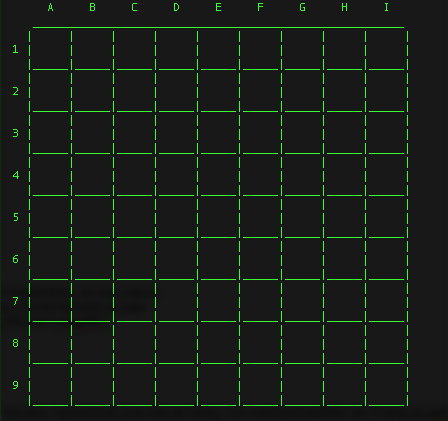
\includegraphics[scale = 0.6]{images/inicial.png}
	\caption{Estado Inicial do Tabuleiro na consola}
	\label{fig:estado_inicial}
\end{figure}

%%Intermedio
\textbf{Representação de um estado intermédio do tabuleiro:}
\linebreak
\lstinputlisting[language=Prolog, numbers=left, firstline=12, lastline=21, breaklines=true, showstringspaces=false, frame=single, columns=flexible]{../src/dristrify.pl}

\begin{figure}[H]
	\centering
	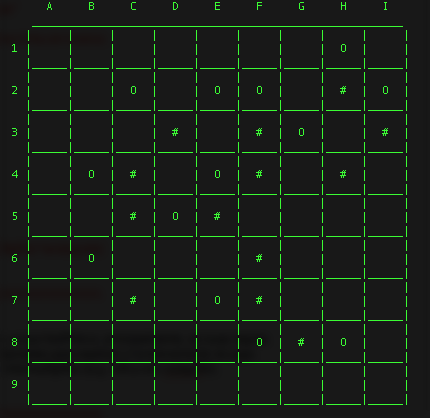
\includegraphics[scale = 0.6]{images/intermedio.png}
	\caption{Um Estado Intermédio do tabuleiro na consola}
	\label{fig:estado_intermedio}
\end{figure}
\newpage
%%Final
\textbf{Representação de um estado final do tabuleiro:}
\linebreak
\lstinputlisting[language=Prolog, numbers=left, firstline=23, lastline=32, breaklines=true, showstringspaces=false, frame=single, columns=flexible]{../src/dristrify.pl}

\begin{figure}[H]
	\centering
	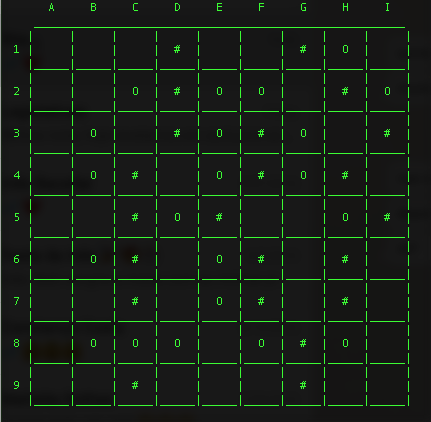
\includegraphics[scale = 0.5]{images/final.png}
	\caption{Um Estado Final do Tabuleiro na consola}
	\label{fig:estado_final}
\end{figure}

\newpage
%%%%%%%%%%%%%%%%%%%%%%%%%%
\section{Visualização do Tabuleiro}

%Descrever a forma de visualização do tabuleiro em modo de texto e o(s) predicado(s) Prolog construídos para o efeito.
%Deve ser incluída pelo menos uma imagem correspondente ao output produzido pelo predicado de visualização.

Para obter a visualização de um tabuleiro basta utilizar o predicado Prolog  \textbf{printBoard(Board)}. Por sua vez, este utiliza os seguintes predicados: 
\linebreak\
\lstinputlisting[language=Prolog, numbers=left, firstline=34, lastline=53, breaklines=true, showstringspaces=false, frame=single, columns=flexible]{../src/dristrify.pl}
A chamada deste predicado produz então o seguinte  \textit{output}:
\begin{figure}[H]
    \centering
    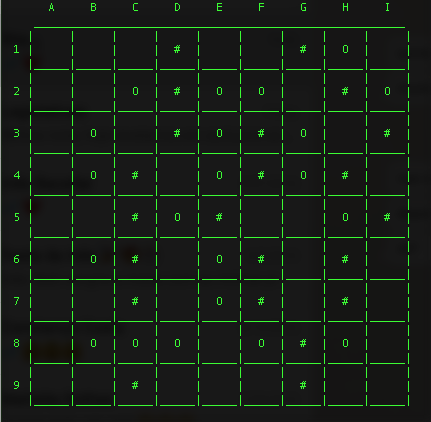
\includegraphics[scale = 0.4]{images/final.png}
    \caption{Output do predicado de visualização}
    \label{fig:final_board}
\end{figure}

\newpage
%%%%%%%%%%%%%%%%%%%%%%%%%%
\section{Movimentos}

%Elencar os movimentos (tipos de jogadas) possíveis e definir os cabeçalhos dos predicados que serão utilizados (ainda não precisam de estar implementados).

Em cada movimento o jogador pode colocar duas peças no tabuleiro. Para isso basta utilizar o seguinte predicado Prolog:
\linebreak
\linebreak
\centerline{placePiece(Board, Player, Row, Column, NewBoard).}
\linebreak
\linebreak\
A variável Board é uma lista de listas com o actual estado do jogo. A variável Player é uma variável que nos indica que jogador está a colocar a sua peça no tabuleiro. Row e Column indicam em que posição no tabuleiro irá ser colocada a peça. Já a NewBoard é a variável que irá conter o novo estado do jogo.


\end{document}
